\chapter{Analyse van Observatieprestaties}
\label{ch:analyse}

\section{Inleiding}

In de voorgaande hoofdstukken werden de ontwikkeling van de PoC applicatie, de methodologie voor het verzamelen 
van experimentele data, en het creëren van een grondwaarheidsdataset uitvoerig besproken. 
Dit hoofdstuk richt zich op de kern van het onderzoek: de geautomatiseerde analyse van de 
observatieprestaties van studenten aan de hand van de verzamelde eyetracking-opnames.

Het hoofddoel van de hier beschreven analyse is, om op basis van de videofeed en blikdata van de Tobii Pro Glasses 3, 
automatisch te bepalen (1) welke van de vooraf gedefinieerde kritische objecten door een student zijn waargenomen en (2) 
hoe lang de aandacht op elk van deze objecten gericht was. 
Om dit te realiseren, werd een analysepipeline ontworpen en geïmplementeerd, die de output van verschillende computervisiemodellen combineert.

De ontwikkelde analysepipeline, zoals conceptueel voorgesteld in Strategie 4 van Hoofdstuk~\ref{ch:oplossingsstrategieen}, 
transformeert de ruwe video- en blikdata, frame-per-frame tot een identificatie van bekeken, kritische objecten. 
Dit proces omvat drie hoofdfasen: (1) het segmenteren en tracken van alle potentiële objecten in beeld, 
(2) het filteren van deze segmenten op basis van objectgrootte en daadwerkelijke observatie door de student, en 
(3) het classificeren van de overgebleven objectsegmenten. 
Er werden drie verschillende benaderingen voor de classificatiestap geëvalueerd:
\begin{enumerate}
  \item \textbf{Vector-Index Classificatie:} Hierbij worden eerst image embeddings van de bekeken segmenten gegenereerd met DINOv2.
  Hierna worden deze embeddings vergeleken met voorbeelden van de kritische objecten binnen een \texttt{Faiss (Facebook AI Similarity Search)} vector-index.
  \item \textbf{YOLOv11 Classificatie:} In deze benadering wordt een YOLOv11-model getraind om de segmenten te classificeren.
  \item \textbf{YOLOv11 Object Detectie:} Deze aanpak verschilt van de vorige doordat het model niet enkel classificeert, 
  maar ook de locatie van de objecten in het frame bepaalt. 
  De objectdetector genereert bounding boxes, die vervolgens worden gecombineerd met de trackingresultaten van FastSAM om tot een definitieve classificatie te komen van elk bekeken object.
\end{enumerate}
Merk op dat het bij de eerste fase niet enkel over frame-per-frame segmentatie gaat, maar ook over het tracken van deze segmenten doorheen de video.
Deze aanpak maakt het mogelijk om na classificatie van de individuele segmenten, de resultaten te aggregeren over de volledige tracking-sessie van elk object. 

De ontwikkelde methoden werden beoordeeld aan de hand van de in Hoofdstuk~\ref{ch:grondwaarheid} gecreëerde grondwaarheid.

Figuur~\ref{fig:analyse-pipeline-visualisatie} illustreert de fasen van dit proces aan de hand van illustratieve beelden.

\begin{figure}[H]
    \centering
        \begin{subfigure}[b]{0.75\textwidth}
        \centering
        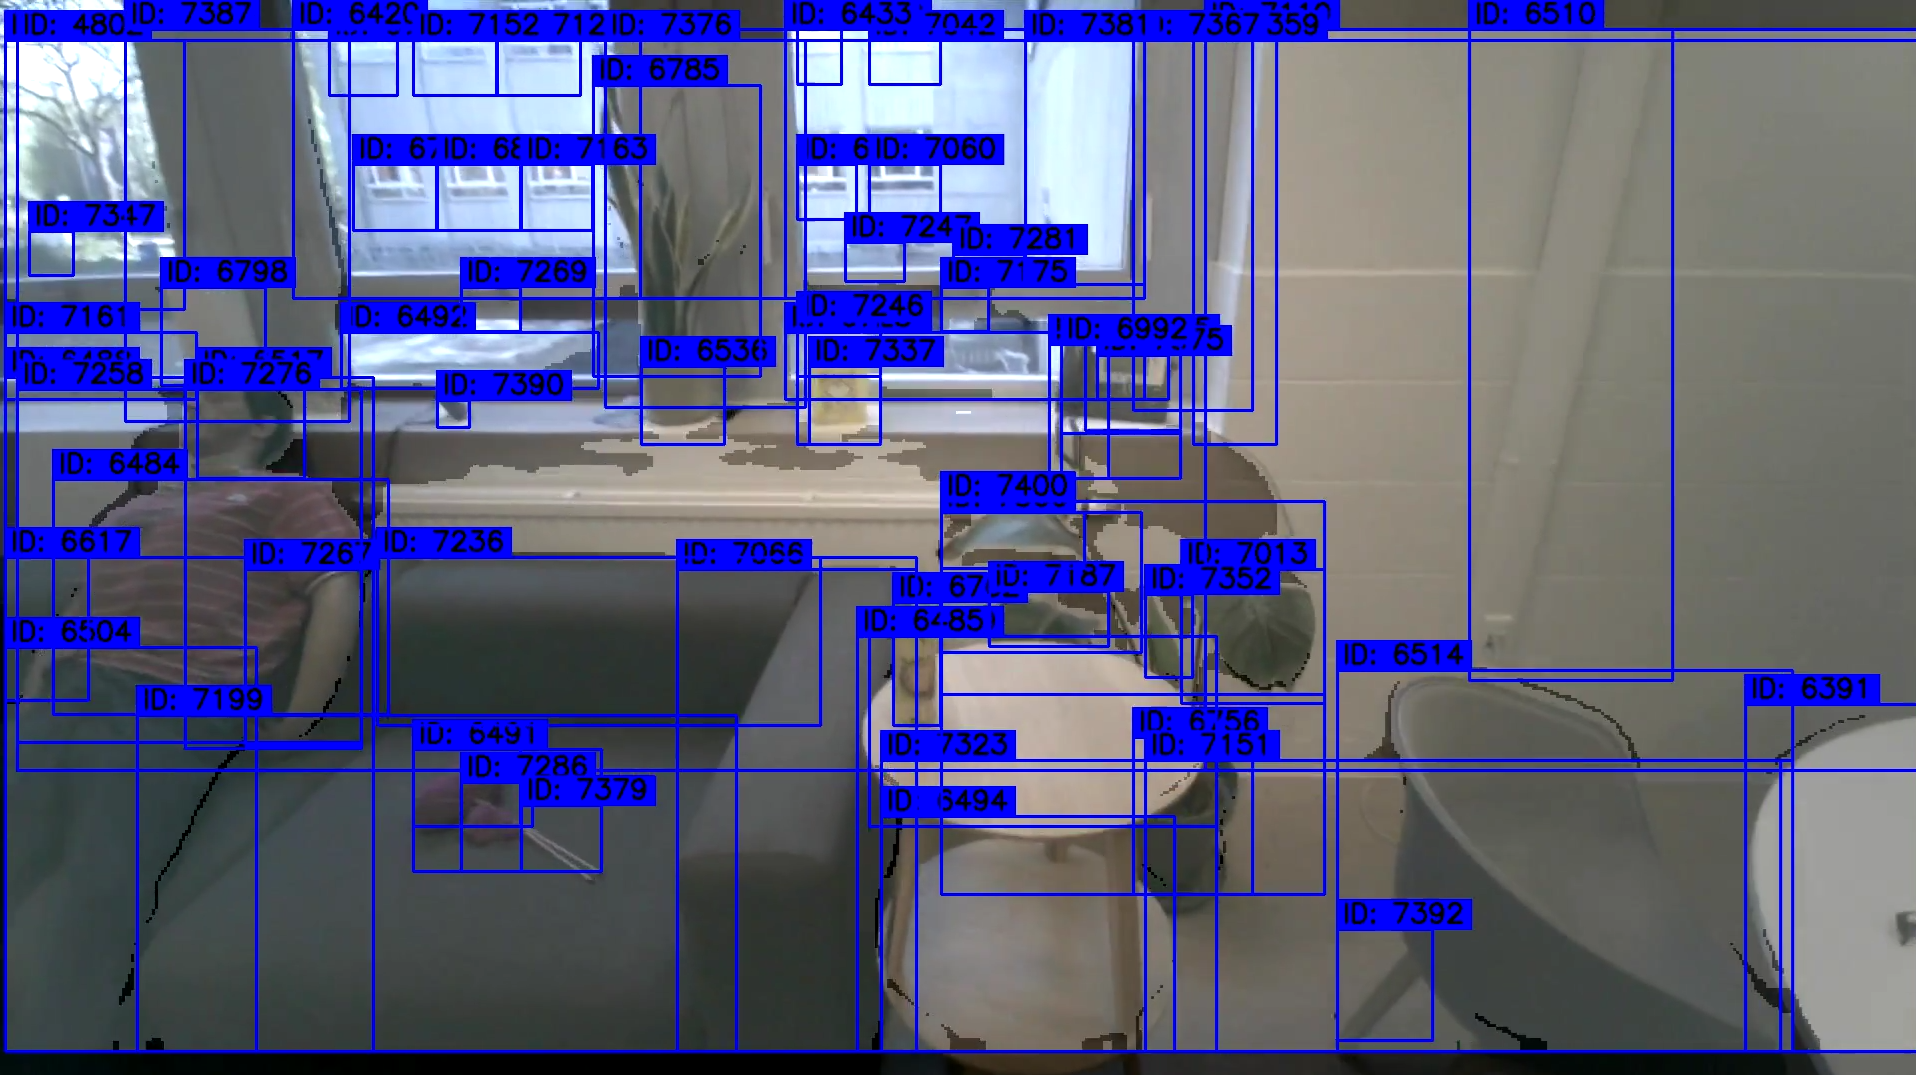
\includegraphics[width=1\textwidth]{everything-prompt.png}
        \caption{Everything-Segmentatie (FastSAM)}
        \label{fig:pipeline_stap_a}
    \end{subfigure}

    \vspace{0.5cm}

    \begin{subfigure}[b]{0.75\textwidth}
    \centering
    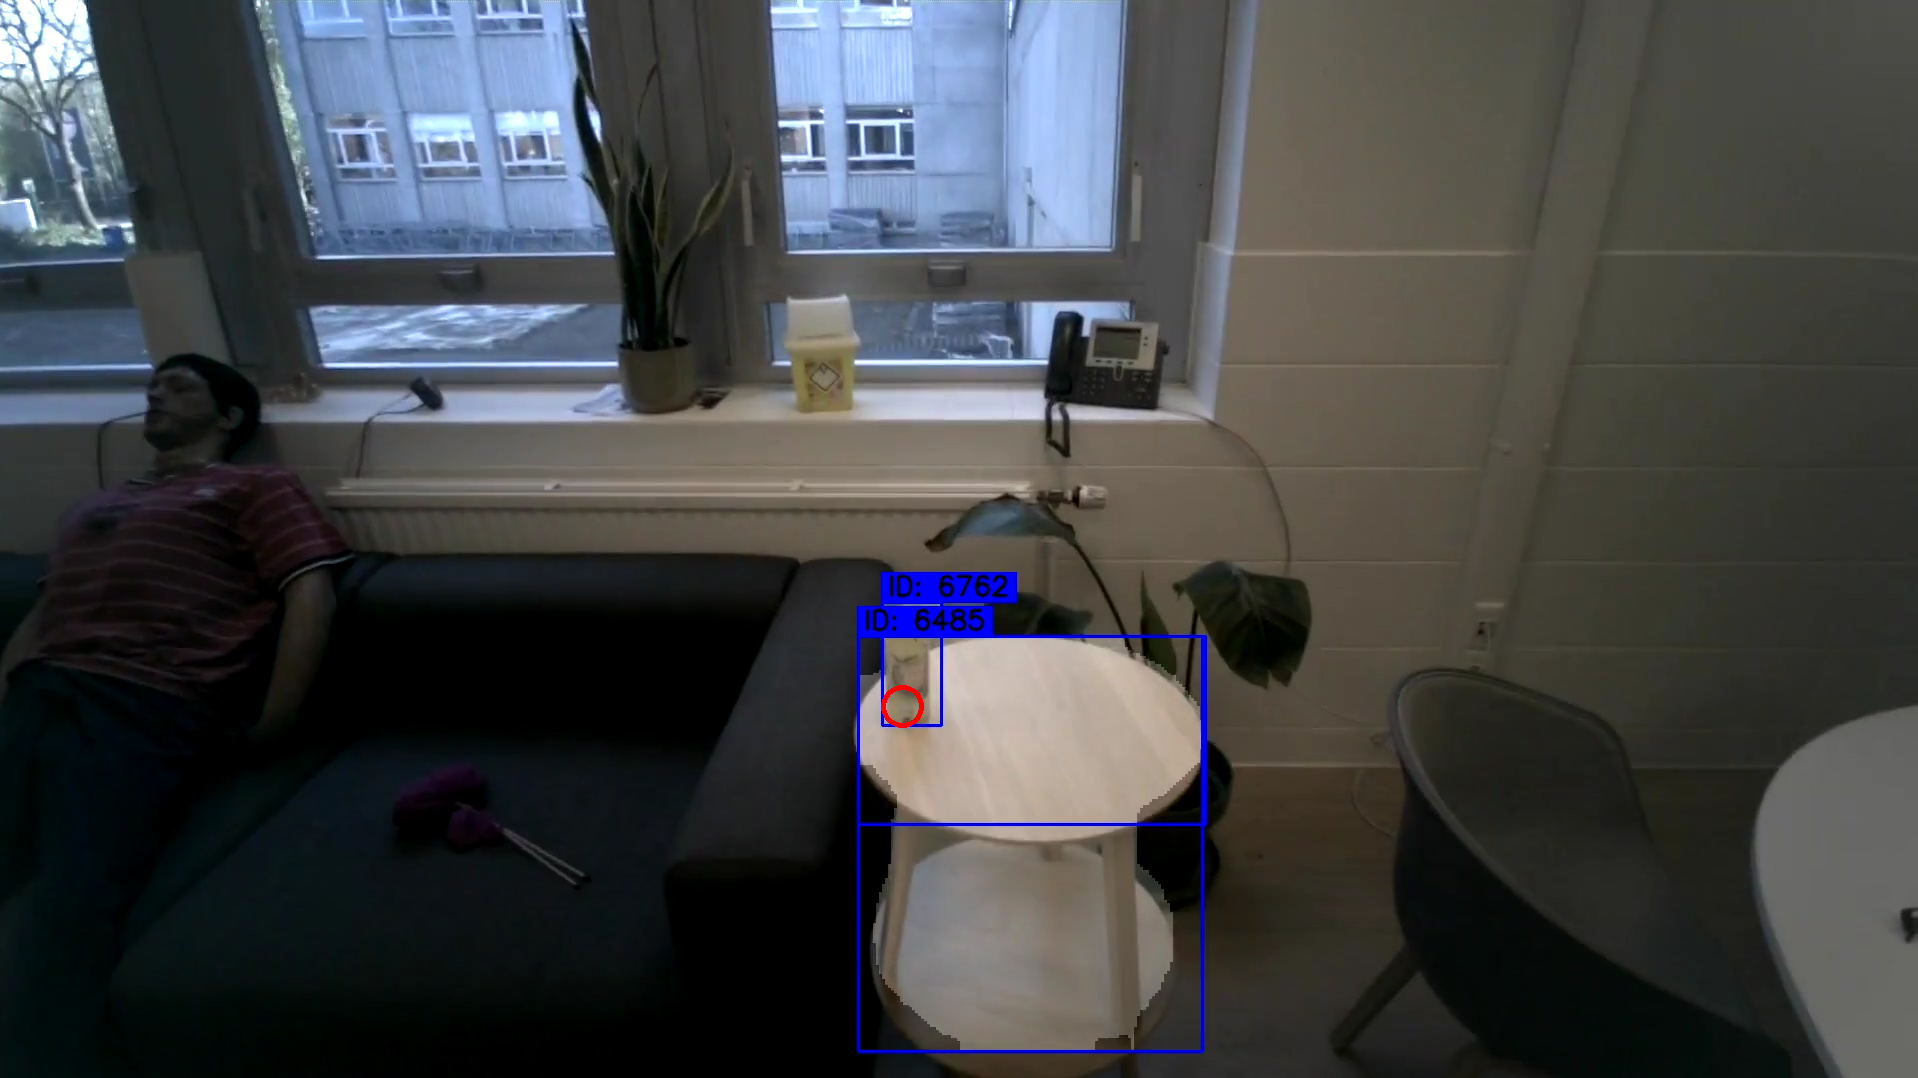
\includegraphics[width=1\textwidth]{filtered-segmentation.png}
    \caption{Filtering op basis van blikpunt en objectgrootte}
    \label{fig:pipeline_stap_b}
    \end{subfigure}

    \vspace{0.5cm}

    \begin{subfigure}[b]{0.75\textwidth}
        \centering
        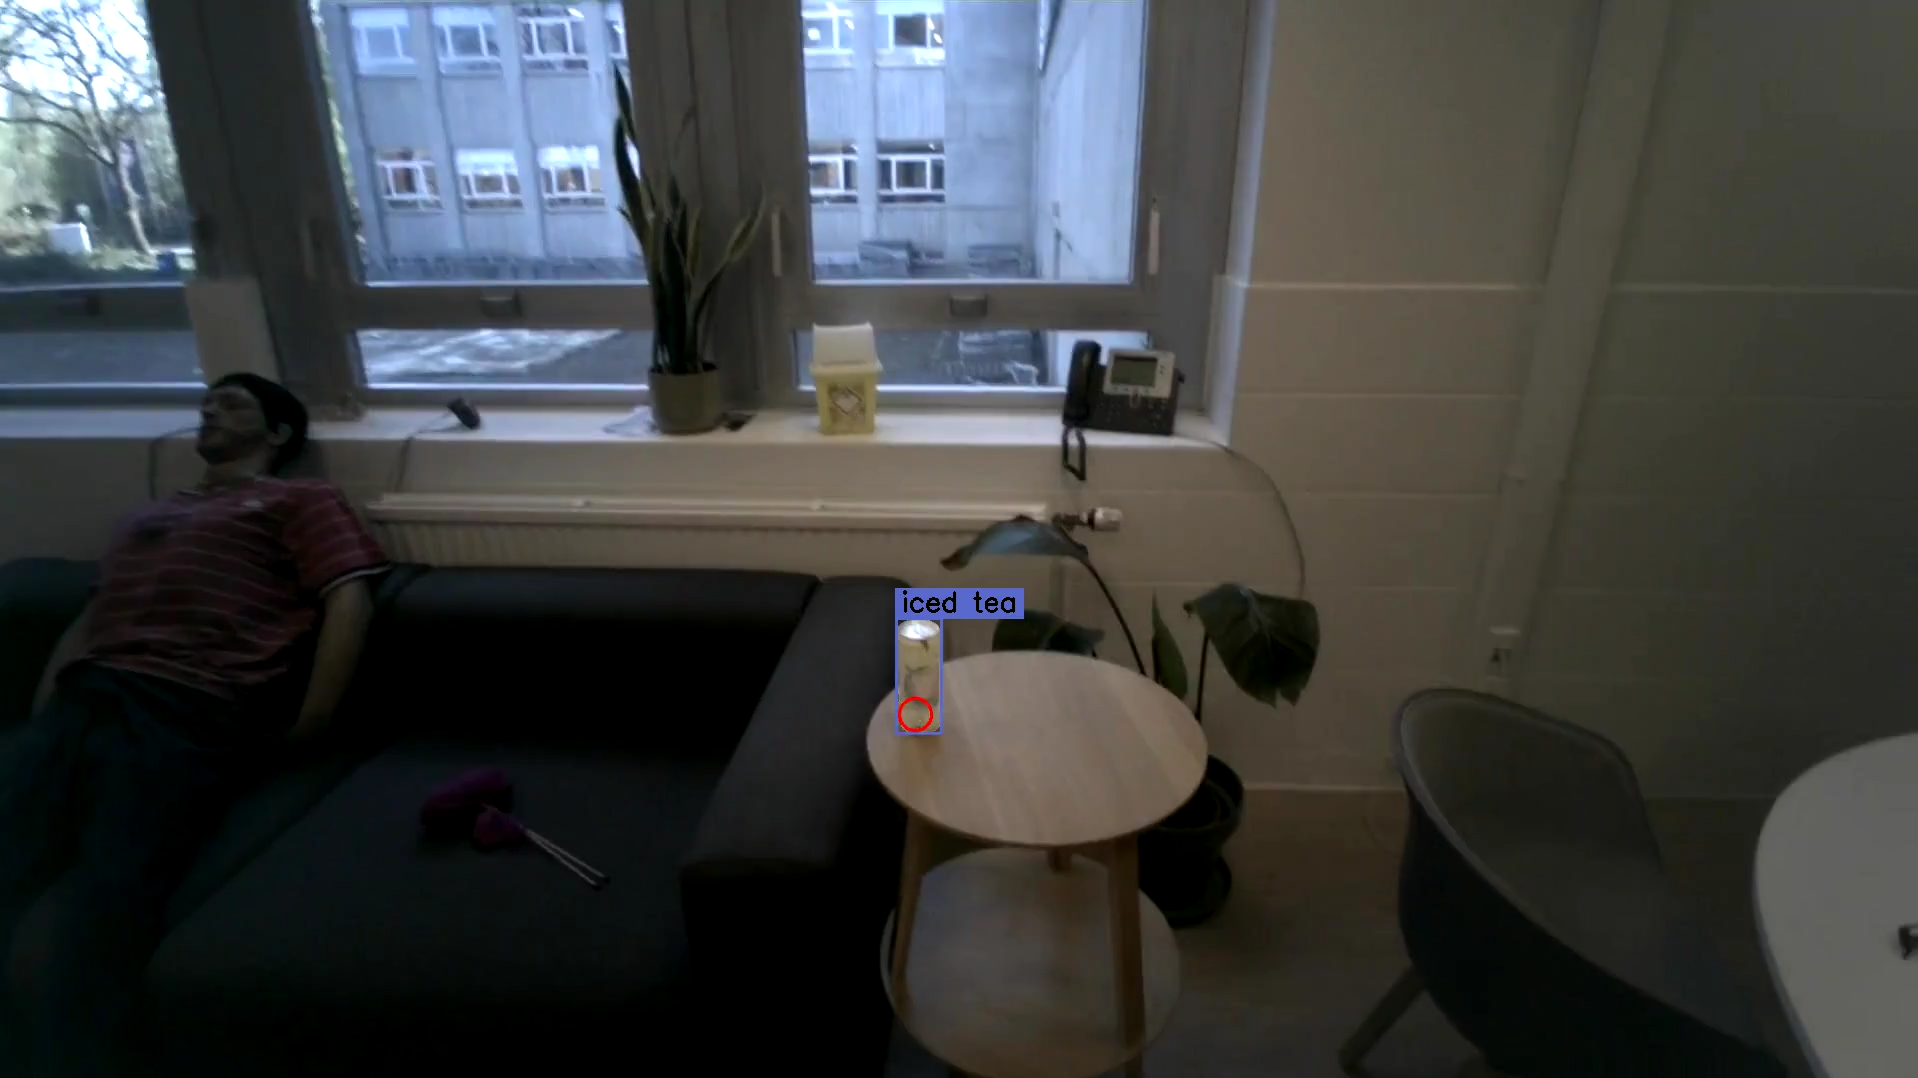
\includegraphics[width=1\textwidth]{classification-example.png}
        \caption{Classificatiestap}
        \label{fig:pipeline_stap_c}
    \end{subfigure}
    \caption[Visualisatie van de Analysepipeline]{
        \label{fig:analyse-pipeline-visualisatie}
        Visualisatie van de stappen in de analysepipeline.
        (\subref{fig:pipeline_stap_a}) FastSAM segmenteert alle objecten in het beeld en volgt deze doorheen de video.
        (\subref{fig:pipeline_stap_b}) De segmenten worden gefilterd; enkel de segmenten die daadwerkelijk met de blik van de gebruiker overlappen worden behouden.
        (\subref{fig:pipeline_stap_c}) De overgebleven segmenten worden uit de originele frame geknipt en dienen als input voor een classificatiemodel.
    }
\end{figure}

\section{Tracking en Segmentatie van Objecten}

De eerste fase van de analysepipeline is erop gericht om uit de continue videostroom alle potentieel relevante objectregio's 
te isoleren die daadwerkelijk door de student zijn bekeken. 
De implementatie van dit proces werd vastgelegd in de python-notebook \texttt{04\_gaze\_segmentation.ipynb},
en wordt hieronder toegelicht.
De besproken code binnen deze fase is terug te vinden in de \texttt{GazeSegmentationJob} klasse in de notebook.

Voor deze fase werd gekozen om gebruik te maken van het FastSAM-model, vanwege zijn hoge snelheid.
Dit maakte het mogelijk om snel de aanpak te optimaliseren en de pipeline te testen, zonder dat de tijdsduur van de analyse een beperkende factor werd.
Het model komt in twee varianten: een `large' (\texttt{FastSAM-x}) en een `small' (\texttt{FastSAM-s}) versie.
Er werd gekozen om de `large' versie te gebruiken, vanwege de betere segmentatiekwaliteit.
FastSAM is beschikbaar via de \texttt{ultralytics}\footnote{\url{https://docs.ultralytics.com/models/fast-sam/}} python-bibliotheek,
die een \texttt{track} functie bevat die het mogelijk maakt om alle objecten in een video zowel te segmenteren als te tracken.

\subsection{Tracking en Segmentatie van Objecten}

In een eerste stap worden alle frames van de evaluatieopname geëxtraheerd naar een tijdelijke map met behulp van \texttt{ffmpeg}.
Daarna is het mogelijk om de \texttt{track} functie toe te passen op deze frames:

\begin{listing}[H]
  \begin{minted}{python}
    frame_paths = list(self.frames_path.iterdir())
    # Frames sorteren op basis van hun naam (index)
    frame_paths.sort(key=lambda x: int(x.stem))

    for frame_path in frame_paths:
        frame_idx = int(frame_path.stem)
        results = self.model.track(
            source=str(frame_path), imgsz=1024, verbose=False, persist=True
        )[0]
    \end{minted}
  \caption[Tracking van objecten met FastSAM]{}
\end{listing}

Hier zijn volgende zaken belangrijk om op te merken:
\begin{itemize}
    \item De frames dienen gesorteerd te worden op basis van hun volgorde in de video.
    \item De \texttt{track} functie neemt een parameter \texttt{imgsz} aan, die de grootte van de inputafbeeldingen bepaalt.
    Indien de afbeeldingen te groot of te klein zijn, worden ze automatisch geschaald.
    Deze parameter heeft zowel invloed op de snelheid van de segmentatie als op de kwaliteit ervan.
    \item Het is belangrijk om de \texttt{persist} parameter op \texttt{True} te zetten, 
    zodat het model de tracking-informatie kan behouden tussen opeenvolgende frames.
    \item De \texttt{track} functie levert een lijst op van \texttt{Results}-objecten, maar bevat hier slechts één element, aangezien de functie telkens een enkele frame behandelt.
    Dit \texttt{Results}-object bevat de segmentatiemaskers, bounding boxes, en tracking-informatie voor elk object in het frame.
\end{itemize}

% TODO: IOU? CONF?

\subsection{Filteren van Tracking-Resultaten}

Na het uitvoeren van de tracking en segmentatie, worden de resultaten gefilterd op basis van twee criteria:
\begin{itemize}
    \item \textbf{Objectgrootte:} Segmenten die een onrealistisch groot deel van het beeld beslaan (bijvoorbeeld muren, vloeren, of de gehele achtergrond) worden weggelaten.
    \item \textbf{Blikdata:} Met behulp van de \texttt{mask\_was\_viewed} functie (zie Sectie~\ref{sec:filtering-annotaties}) 
    wordt voor elk overgebleven segment gecontroleerd of het blikveld van de student daadwerkelijk overlapt met het segmentatiemasker in dat specifieke frame. 
    Enkel de `bekeken' segmenten worden behouden voor verdere analyse.
\end{itemize}

Hier zullen we enkel de \texttt{mask\_too\_large} functie toelichten.
Codefragment~\ref{listing:filteren-segmenten-grootte} toont de implementatie hiervan.

\begin{listing}[H]
  \begin{minted}{python}
    def mask_too_large(self, mask: torch.Tensor) -> bool:
        MAX_MASK_AREA = 0.1
        height, width = mask.shape
        frame_area = height * width
        max_mask_area = MAX_MASK_AREA * frame_area

        mask_area = mask.sum()
        return mask_area >= max_mask_area
    \end{minted}
  \caption[Filteren van segmenten op basis van grootte]{
    \label{listing:filteren-segmenten-grootte}  
    Deze functie controleert of een segment te groot is op basis van de oppervlakte van het segmentatiemasker. 
  }
\end{listing}

Hier wordt een som berekend van alle pixels in het segmentatiemasker (aangezien het masker binair is).
Indien deze som groter is dan de maximaal toegestane oppervlakte, wordt het masker als `te groot' beschouwd.
De maximale oppervlakte van een segment wordt gedefinieerd als 10\% van de totale oppervlakte van het frame.
Dit is momenteel een arbitraire waarde, maar kan in de toekomst verder geoptimaliseerd worden, of zelfs 
dynamisch worden ingesteld op basis van objecten binnen kalibratieopnames in de applicatie.

\subsection{Opslaan van de Resultaten}

Na het filteren van de segmenten, worden de resultaten van elke frame opgeslagen in gecomprimeerde numpy-bestanden 
(\texttt{.npz}) onder \texttt{data/gaze\_segmentation\_results}.

\begin{listing}[H]
  \begin{minted}{python}
    executor.submit(
        np.savez_compressed,
        self.results_path / f"{frame_idx}.npz",
        boxes=boxes,
        rois=rois_array,
        masks=masks_array,
        object_ids=object_ids,
        frame_idx=frame_idx,
        gaze_position=gaze_position,
        confidences=confidences,
    )
    \end{minted}
  \caption[Opslaan van segmentatie-resultaten]{
    \label{listing:opslaan-segmentatie-resultaten}
    Deze code slaat de resultaten van de segmentatie en tracking op in een gecomprimeerd numpy-bestand.
    De resultaten worden opgeslagen per frame, met de relevante metadata.
  }
\end{listing}

De volgende gegevens worden opgeslagen:
\begin{itemize}
    \item \textbf{boxes:} De bounding boxes van de segmenten, handig voor het visualiseren van de segmenten in de video.
    \item \textbf{rois:} De ROI's (Region of Interest) van de segmenten. Deze worden later gebruikt bij de classificatiestap om de objecten te identificeren.
    \item \textbf{masks:} De segmentatiemaskers van de objecten, die ook worden gebruikt voor visualisatie.
    \item \textbf{object\_ids:} De unieke ID's van de objecten, die worden toegewezen door het FastSAM-model. Deze ID's blijven consistent voor elk specifiek object over meerdere frames,
    tenzij de tracking verloren gaat (bijvoorbeeld wanneer het object tijdelijk uit beeld is). Wanneer dit gebeurt, wordt een nieuwe ID toegewezen aan het object als het opnieuw in beeld komt.
    Deze ID maakt het mogelijk om de resultaten van de classificatiestap te aggregeren over meerdere frames, om zo een beter resultaat te krijgen.
    \item \textbf{frame\_idx:} De index van het frame, die wordt gebruikt om de resultaten te koppelen aan het juiste frame in de video.
    \item \textbf{gaze\_position:} De blikpositie van de student in dat specifieke frame (indien beschikbaar).
    \item \textbf{confidences:} De vertrouwensscore van het model voor elk segment, die aangeeft hoe zeker het model is dat het segment correct is.
    Dit kan nuttig zijn voor het filteren van segmenten die een lage vertrouwensscore hebben, 
    of het vinden van correlaties tussen de vertrouwensscore en de uiteindelijke classificatie.
\end{itemize}
Aangezien het opslaan van de resultaten IO-intensief is, wordt dit proces uitgevoerd met behulp van multithreading (\texttt{executor.submit}).

\subsection{Voorbereiding van de Tracking Resultaten voor Classificatie}

De output van de vorige stap bestaat uit een reeks \texttt{.npz}-bestanden, één per frame, 
die de gefilterde segmenten, ROIs, en bijbehorende metadata bevatten. 
Om deze data efficiënt te kunnen gebruiken als input voor de classificatiestrategieën, werd een aanvullende voorbereidingsstap uitgevoerd. 
Deze stap werd geïmplementeerd in de notebook \texttt{05\_create\_object\_datasets.ipynb} en consolideert de frame-per-frame 
resultaten tot een gestructureerde dataset per evaluatieopname. 
Deze dataset, hierna `object-dataset' genoemd, aggregeert alle metadata van de bekeken segmenten binnen een enkele tabel.
Hoewel veel van deze metadata ook in de individuele \texttt{.npz}-bestanden te vinden zijn, resulteert de consolidatie 
naar één \texttt{.csv}-bestand per opname in een efficiëntere dataverwerking tijdens de classificatiefase. 
Het vermijdt het herhaaldelijk openen en parsen van potentieel honderden of duizenden afzonderlijke \texttt{.npz}-bestanden.

Het creëren van de object-dataset omvat het itereren over de \texttt{.npz}-bestanden van elke opname. 
Voor elk gedetecteerd en gefilterd object (ROI) binnen een frame worden de volgende kenmerken geëxtraheerd en samengevoegd tot een rij in een \texttt{Pandas DataFrame}:
\begin{itemize}
    \item \texttt{frame\_idx}: De index van het frame waarin het object oorspronkelijk werd gedetecteerd. 
    Dit koppelt het object aan een specifiek tijdstip in de video.
    \item \texttt{object\_id}: De unieke, tijdelijke ID die door het FastSAM-model aan het getrackte object 
    is toegewezen binnen de scope van die specifieke tracking-sessie.
    \item \texttt{confidence}: De vertrouwensscore van het FastSAM-model voor de detectie van dit specifieke segment. 
    Deze score geeft een indicatie van hoe zeker het model was van zijn segmentatie.
    \item \texttt{embedding}: Een dense vectorrepresentatie (embedding) van de visuele kenmerken van de ROI, 
    gegenereerd met het DINOv2-model. 
    Deze embedding dient als input voor de op similariteit gebaseerde classificatie met een vector-index.
    Meer hierover in de volgende sectie.
    \item \texttt{mask\_area}: De totale oppervlakte van het segmentatiemasker van het object in pixels. 
    Dit geeft een maat voor de (schijnbare) grootte van het object in het frame.
    \item \texttt{x1, y1, x2, y2}: De coördinaten die de bounding box rondom het gedetecteerde object definiëren. 
\end{itemize}

De resulterende \texttt{DataFrame} wordt vervolgens opgeslagen 
als een \texttt{.csv}-bestand onder \texttt{data/object\_datasets/<recording\_id>}. 
Het resultaat is een set van tabelvormige datasets die klaar zijn voor de daadwerkelijke classificatietaken.

\section{Classificatie van Objecten}

De vorige fase leverde een dataset op met bekeken objectsegmenten (ROIs) per evaluatieopname.
Deze kregen echter nog geen label toegewezen, dat aangeeft tot welk van de kritische objecten ze behoren.
Om dit te realiseren, werd een classificatiestap geïmplementeerd die de ROIs labelt op basis van hun visuele kenmerken.

\subsection{Data Labeling}

Voor het initialiseren en trainen van de classificatiestrategieën was het noodzakelijk om een dataset te hebben met gelabelde objecten.
Zoals eerder beschreven in Hoofdstuk~\ref{ch:experiment} (Sectie~\ref{sec:kalibratieopnames}), werden hiertoe 
twee specifieke kalibratieopnames gemaakt door de onderzoeker.
De eerste opname bevatte de objecten in hun oorspronkelijke posities en achtergrond, identiek aan de evaluatieopnames.
De tweede opname toonde dezelfde objecten tegen een significant afwijkende achtergrond, 
primair bedoeld om de invloed van contextvariatie te onderzoeken.

Bij de analyses die in dit hoofdstuk worden gepresenteerd, is uitsluitend gebruik gemaakt 
van de data uit de kalibratieopname met de originele achtergrond.
De beslissing om de tweede kalibratieopname buiten beschouwing te laten, werd genomen om de scope van deze bachelorproef beheersbaar te houden.
Een discussie over het potentieel van deze tweede dataset voor verder onderzoek is terug te vinden in Hoofdstuk~\ref{ch:conclusie}.
% TODO: toevoegen aan conclusie

\paragraph{Labeling voor Classificatie}
Voor de initiële, op ROI-gebaseerde classificatiepogingen, was de labelingstrategie relatief eenvoudig.
Het volstond om voor elk van de objecten een representatief aantal ROIs te verzamelen en te labelen gedurende de 
tijdsvensters van 30 seconden waarin elk object centraal werd bekeken. 
Dit leverde voldoende voorbeelden van elk object op voor het trainen van de classificatiemodellen.

\paragraph{Labeling voor Objectdetectie}
Voor het trainen van het objectdetectiemodel was echter een meer omvattende aanpak vereist.
In tegenstelling tot ROI-classificatie die op geïsoleerde objectsegmenten werkt, wordt een objectdetector 
getraind om objecten te lokaliseren binnen een breder beeld.
Tijdens de training analyseert het model `crops' (vierkante regio's van het beeld) en leert het model om objecten te detecteren binnen zulke regio's.
Hierbij is het belangrijk dat binnen de labeling alle objecten in het beeld worden gemarkeerd, die potentieel binnen een crop kunnen vallen
(zie Figuur~\ref{fig:voorbeeld_crop_yolo_training} voor een conceptuele visualisatie van een crop).
De manier waarop deze crops worden gedefinieerd binnen de trainingsdataset, komt later in dit hoofdstuk aan bod.
% TODO: verwijzen naar sectie

\begin{figure}[H]
    \centering
    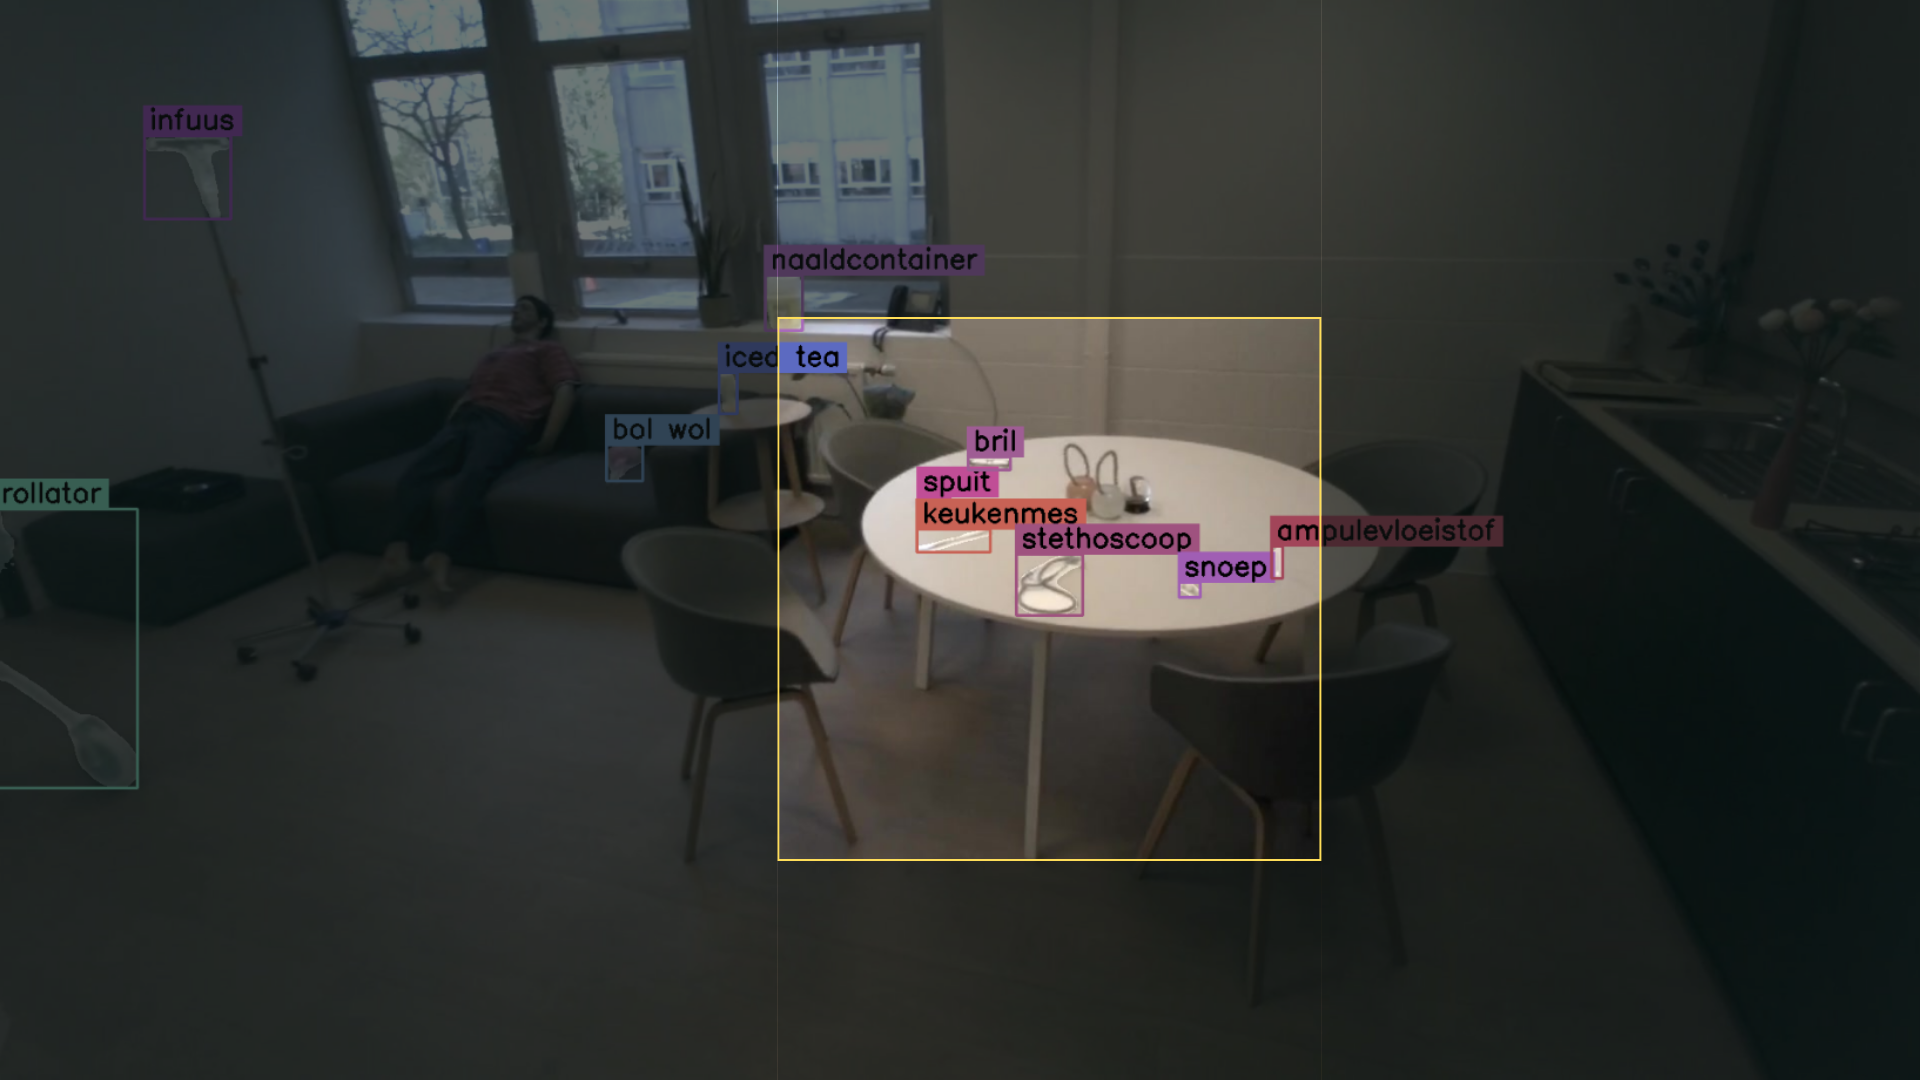
\includegraphics[width=1\textwidth]{yolo_training_crop.png}
    \caption[Voorbeeld van een crop voor objectdetectie]{
        \label{fig:voorbeeld_crop_yolo_training}
        Voorbeeld van een frame uit de labeling tool. 
        Hier wordt een voorbeeld van een crop getoond die gebruikt kan worden voor het trainen van een objectdetectiemodel.
        Het is dus belangrijk dat alle objecten die binnen deze crop kunnen vallen,
        worden gelabeld, zelfs als ze niet volledig zichtbaar zijn.
        Merk op dat dit niet de enige mogelijke crop is binnen deze afbeelding, men kan ook andere regio's selecteren met andere objecten.
    }
\end{figure}

\paragraph{Opmerking: Ampule Poeder Niet Gelabeld}
Het object `ampule poeder' werd in de labeling niet opgenomen. 
Origineel werd het object gekozen omwille van zijn doorschijnende karakter (glazen ampule).
Het werd ook naast een andere groep objecten geplaatst om de detectie alsnog te bemoeilijken (zie Figuur~\ref{fig:ampulepoeder}).
Echter, tijdens de labeling bleek het object te moeilijk voor het SAM2 model om te segmenteren en te tracken.
Dit resulteerde in een lage labelingkwaliteit, waarbij de segmenten inaccuraat waren.
Soms werden zelfs ook foutief aangrenzende objecten meegenomen in de segmentaties.
Om deze reden werd besloten om het object niet mee te nemen in de labeling en de uiteindelijke analyse. 
Een ander object, de `ampule vloeistof', werd wel opgenomen ondanks zijn sterk doorschijnende karakter.
Dit object bleek veel gemakkelijker te volgen en te segmenteren door het FastSAM-model, vermoedelijk omdat het afgezonderd was van andere, 
potentieel verwarrende objecten.

\begin{figure}[H]
    \centering
    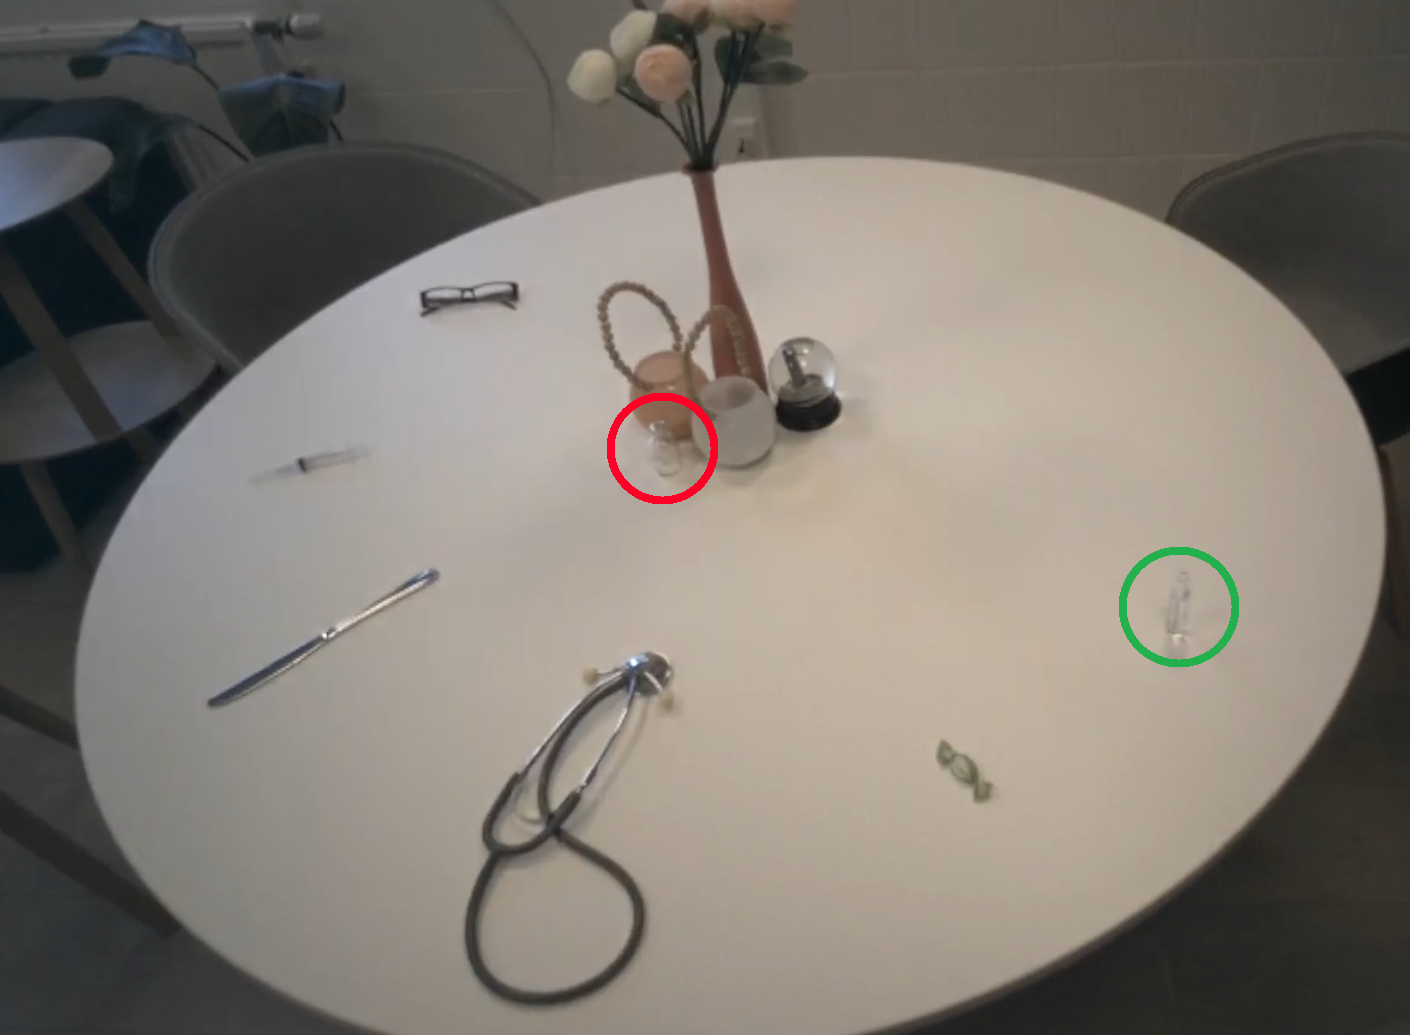
\includegraphics[width=0.8\textwidth]{ampulepoeder.png}
    \caption[Voorbeeld van de ampule poeder in de kalibratieopname]{
        \label{fig:ampulepoeder}
        Locatie van de ampule poeder in de kalibratieopname, aangeduid met een rode cirkel.
        De ampule vloeistof werd wel opgenomen in de labeling, en is hier aangeduid met een groene cirkel.
    }
\end{figure}

\subsection{Initiële Classificatiepogingen en Uitdagingen}

Nadat de object-datasets waren aangemaakt en de referentiedata uit de kalibratieopname was gelabeld, was de volgende stap het 
toewijzen van een label aan elk gedetecteerd en door de student bekeken objectsegment (ROI). 
Er werden initieel twee strategieën onderzocht voor het classificeren van deze ROIs, waarvan de relevante data beschikbaar waren in de object-datasets:
\begin{enumerate}
    \item \textbf{Vector-Index Classificatie:} Hierbij werden de DINOv2-embeddings van de ROIs vergeleken met referentie-embeddings van de kritische objecten afkomstig uit de kalibratieopname.
    Er werd een Faiss (Facebook AI Similarity Search) index gebruikt om de meest vergelijkbare referentie-embeddings te vinden.
    Faiss is een bibliotheek die het mogelijk maakt om snel zoekopdrachten uit te voeren op grote datasets van vectoren.
    \item \textbf{YOLOv11 Classificatie:} Een YOLO-model werd getraind, niet voor detectie in het volledige frame, maar specifiek voor het classificeren van de reeds 
    geïsoleerde ROIs uit de evaluatieopnames.
\end{enumerate}

Deze twee benaderingen zullen hier echter niet diepgaand worden behandeld, 
aangezien beiden al in een vroeg stadium van evaluatie een fundamenteel gebrek vertoonden, 
namelijk een onacceptabel hoge mate van vals-positieven. 
Het probleem lag niet zozeer in de specifieke modelkeuzes, maar in een verkeerde definitie van het classificatieprobleem.
De gekozen classificatietechnieken zijn inherent ontworpen voor \textit{gesloten-set} scenario's. 
In dergelijke scenario's  wordt aangenomen dat elke te classificeren input (elke bekeken ROI)
daadwerkelijk tot één van de vooraf gedefinieerde klassen behoort. 

De realiteit van de observaties is echter complexer en sluit veel beter aan bij het concept van \textit{Open Set Recognition (OSR)}. 
Zoals \textcite{Wang2023} beschrijven in hun overzichtsartikel, is het 
``doorgaans moeilijk om, wanneer men een herkenner of classificator traint, trainingsvoorbeelden te verzamelen die alle (mogelijke) klassen omvatten''.
OSR beschrijft een scenario waarin 
``er ten tijde van de training onvolledige kennis van de wereld bestaat, en onbekende klassen tijdens het testen aan een algoritme kunnen worden voorgelegd''.
Dit vereist dat een classificatiemodel ``niet alleen de geziene klassen accuraat classificeert, maar ook effectief omgaat met de ongeziene'' (citaten uit \textcite{Wang2023}, eigen vertaling).

In de context van dit onderzoek betekende dit dat de studenten talloze objecten en achtergrondelementen bekeken die \textit{niet} tot de kritische objecten behoorden.
De geïmplementeerde ROI-classificatiemodellen waren niet in staat om deze `onbekende' inputs effectief te herkennen en te verwerpen.
In plaats daarvan waren ze geneigd elke ROI te classificeren als één van de objecten, wat resulteerde in de waargenomen overvloed aan vals-positieven.

Gezien deze mismatch tussen de aard van het probleem en de gekozen aanpak, werd besloten deze classificatiestrategieën niet verder te optimaliseren.
De focus verschoof naar een methode die beter is uitgerust om specifieke, bekende objecten te identificeren: objectdetectie.

\section{Objectdetectie met YOLOv11} 

Bij de voorgaande classificatiestrategieën lag de focus op het classificeren van geïsoleerde objectsegmenten afkomstig uit de FastSAM everything-segmentatie.
% TODO: Intro iets beter maken

\subsection{Creatie van de Trainingsdataset voor Objectdetectie}

Gebaseerd op de gelabelde kalibratieopname die eerder werd besproken, werd een specifieke trainingsdataset voor objectdetectie gecreëerd.
Zoals eerder vermeld, werd het object `ampule poeder' niet opgenomen in de labeling, resulterende in een dataset met 14 objecten.
Deze moest bestaan uit beelduitsnedes (hierna `crops' genoemd) waarin de kritische objecten gelabeld zijn met bounding boxes.
De creatie van deze dataset werd geïmplementeerd in de python notebook \texttt{12\_prepare\_object\_detection\_datasets.ipynb}.
Omwille van de beknoptheid zullen in deze sectie enkel de belangrijkste codefragmenten worden getoond; 
de geïnteresseerde lezer wordt verwezen naar de genoemde notebook voor de volledige implementatiedetails van de hieronder beschreven stappen.

\subsubsection{Formaat van de Trainingsdataset}

Alvorens de trainingsdataset te creëren, was het belangrijk om het beoogde formaat van de dataset te bepalen.
Een eerste overweging was de resolutie van de crops. 
Om tot een geïnformeerde keuze te komen, werd een analyse uitgevoerd op de afmetingen van de bounding boxes 
van de gelabelde objecten in de kalibratieopname. 
Figuur~\ref{fig:size-histogram} toont histogrammen van zowel de breedte (links) als de hoogte (rechts) 
in pixels van deze bounding boxes. 
Uit de histogrammen blijkt dat de meerderheid van de objecten een breedte en hoogte heeft van minder dan 400 pixels. 
Enkele objecten, of objecten die van zeer dichtbij zijn opgenomen, vertonen grotere afmetingen. 
Op basis van deze observatie, en rekening houdend met het feit dat objecten in de praktijk 
niet altijd perfect in het midden van een crop zullen liggen, 
werd gekozen voor een vierkante crop-grootte van 640x640 pixels. 
Deze afmeting biedt een ruime marge om de meeste objecten volledig te omvatten, zelfs als ze enigszins 
verschoven zijn ten opzichte van het centrum van de crop. 
Deze grootte is tevens een gangbare inputresolutie voor YOLO-modellen.

\begin{figure}[H]
    \centering
    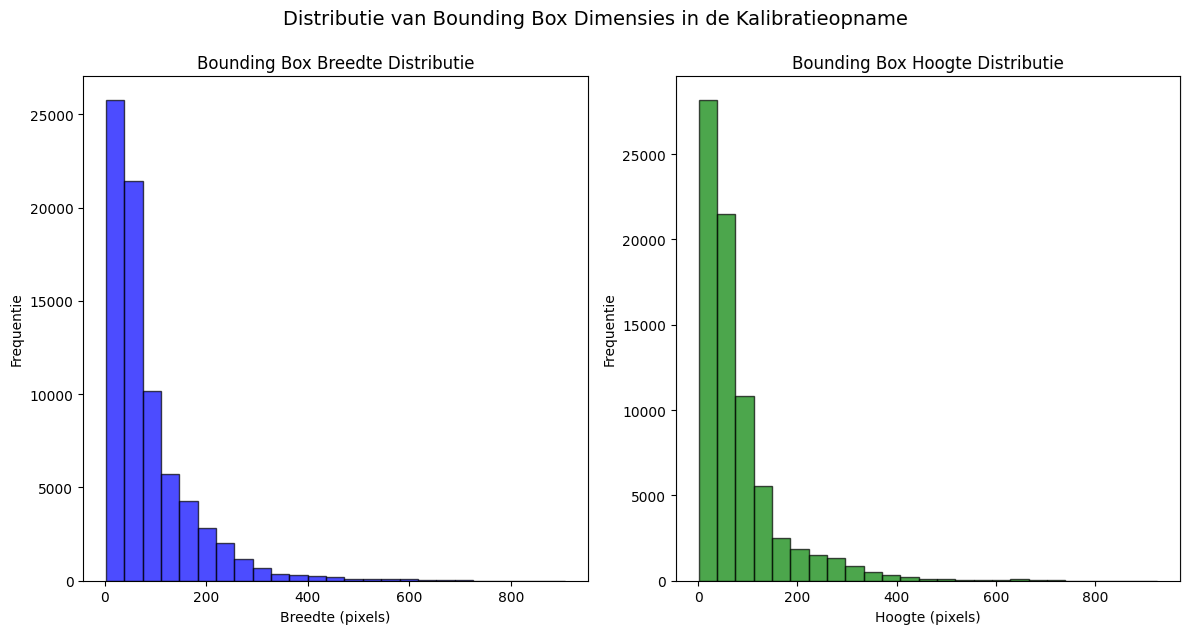
\includegraphics[width=1\textwidth]{bboxes-histogrammen.png}
    \caption[Histogrammen van de breedte en grootte in pixels van bounding boxes in de kalibratieopname]{
      \label{fig:size-histogram}
      Histogrammen van de breedte (links) en hoogte (rechts) in pixels van de bounding boxes in de kalibratieopname.
      De meeste objecten vallen onder de 400 pixels in zowel breedte als hoogte, met een aantal uitzonderingen die groter zijn.
    }
\end{figure}

De volgende overweging betrof de wijze waarop deze crops gegenereerd zouden worden uit de kalibratieopname. 
Aangezien het uiteindelijke doel is om de ROIs die gegenereerd werden door FastSAM, te classificeren, 
dient de trainingsdataset zo goed mogelijk de karakteristieken van deze te classificeren ROIs te weerspiegelen. 
In de praktijk zullen deze ROIs vaak (maar niet altijd perfect) gecentreerd zijn rond het blikpunt van de student, 
omdat de FastSAM-segmentatie en de blikpuntfiltering hierop aansturen. 
Daarom werd voor de creatie van de trainingsdataset besloten om de crops te genereren 
door ze te centreren op het middelpunt van de bounding box van een \textit{geselecteerd doelobject} uit de kalibratieopname. 
Dit simuleert de situatie waarbij het model een ROI aangeboden krijgt waarin het doelobject centraal staat.

Tenslotte vereiste de trainingsdataset voor objectdetectie ook een specifieke structuur, zijnde het \textit{Ultralytics YOLO formaat} (zie Codefragment~\ref{fig:yolo-format}).
% TODO: alle footnotes omvormen naar een bron! \footnote{\url{https://docs.ultralytics.com/datasets/detect/#ultralytics-yolo-format}}

\begin{listing}[H]
  \begin{minted}{text}
    data/
    ├── images/
    │   ├── train/
    │   │   ├── 0000000001.jpg
    │   │   ├── 0000000002.jpg
    │   │   ├── 0000000003.jpg
    │   │   └── ...
    │   └── val/
    │       ├── 0000000001.jpg
    │       ├── 0000000002.jpg
    │       ├── 0000000003.jpg
    │       └── ...
    ├── labels/
    │   ├── train/
    │   │   ├── 0000000001.txt
    │   │   ├── 0000000002.txt
    │   │   ├── 0000000003.txt
    │   │   └── ...
    │   └── val/
    │       ├── 0000000001.txt
    │       ├── 0000000002.txt
    │       ├── 0000000003.txt
    │       └── ...
    └── data.yml
  \end{minted}
  \caption[Voorbeeld van het Ultralytics YOLO Formaat]{
    \label{fig:yolo-format}
    Voorbeeld van de structuur van de trainingsdataset voor objectdetectie in het Ultralytics YOLO formaat.
    De dataset bestaat uit een map met afbeeldingen (in dit geval crops) en een map met labels.
    Elke afbeelding heeft een bijbehorende labelbestand met dezelfde naam, waarin de bounding boxes en klassen van elk object in de afbeelding zijn gedefinieerd.
    Het data.yml bestand bevat de metadata van de dataset, wat later aan bod komt.
  }
\end{listing}

\subsubsection{Genereren van de Trainingsdataset}

Het eigenlijke proces voor het creëren van de trainings- en validatiedatasets werd gecoördineert door de functie \texttt{create\_dataset} 
(zie Codefragment~\ref{listing:create-dataset-overview}). 
Deze functie neemt de metadata van de gelabelde objecten, de geëxtraheerde frames van de kalibratieopname, 
en configuratieparameters zoals de crop-grootte en het gewenste aantal samples per klasse als input.

\begin{listing}[H]
  \fontsize{10pt}{9.6pt}
  \begin{minted}{python}
  def create_dataset(
      per_class_metadata: dict,
      frames: list[Path],
      datasets_path: Path,
      crop_size: int,
      dataset_type: str,
      num_samples_per_class: int,
  ):
      # Definieren van de paden voor de trainings- en validatiedatasets
      # ... Code weggelaten voor beknoptheid ...

      # Samples selecteren per klasse en train/val splitsen
      selected_samples_per_class = select_samples_per_class(
          per_class_metadata, num_samples_per_class
      )
      all_samples_per_frame = get_samples_per_frame(per_class_metadata)
      train_samples_per_class, val_samples_per_class = get_train_val_split(
          selected_samples_per_class, train_ratio=0.8
      )

      # Datasetfiles aanmaken
      class_label_to_model_id = create_metadata_yaml(dataset_path, per_class_metadata)
      create_train_or_val_dataset(
          per_class_metadata,
          class_label_to_model_id,
          train_samples_per_class,
          all_samples_per_frame,
          frames,
          train_images_path,
          train_labels_path,
          crop_size=crop_size,
      )
      create_train_or_val_dataset(
          per_class_metadata,
          class_label_to_model_id,
          val_samples_per_class,
          all_samples_per_frame,
          frames,
          val_images_path,
          val_labels_path,
          crop_size=crop_size,
          is_validation=True,
      )

      return dataset_path
  \end{minted}
  \caption[Functie voor het creëren van de objectdetectie-trainingsdataset]{
    \label{listing:create-dataset-overview}
    De \texttt{create\_dataset} functie coördineert het creëren van de trainings- en validatiedatasets voor objectdetectie.
    Deze functie definieert de paden voor de datasets, maakt de benodigde mappen aan,
    selecteert de samples per klasse, splitst deze in train- en validatiesets,
    en roept de \texttt{create\_train\_or\_val\_dataset} functie aan om de crops en labels te genereren. 
  }
\end{listing}

De benodigde stappen voor het creëren van de trainingsdataset kunnen worden samengevat in drie hoofdfasen, zoals hieronder beschreven.

\paragraph{1. Verzamelen van Metadata per Klasse}

De notebook laadt in een eerste stap de bestandspaden van de trackingresultaten per klasse 
voor de kalibratieopname via de functie \texttt{get\_tracking\_results\_per\_class} (zie voorgaande Codefragment~\ref{listing:opslaan-segmentatie-resultaten}).
Vervolgens worden op basis van de trackingresultaten, metadata per klasse verzameld door de functie \texttt{get\_metadata\_per\_class} aan te roepen.
Dit resulteert in een dictionary waarin elke klasse ID is gekoppeld aan een dictionary met de volgende informatie:
\begin{itemize}
    \item \texttt{class\_name}: De naam van de klasse, bijvoorbeeld `monitor'.
    \item \texttt{color}: Het kleur van de klasse in hexadecimale notatie.
    \item \texttt{frame\_indexes}: Een lijst van frame-indexen waarin de klasse voorkomt in de trackingresultaten.
    \item \texttt{mask\_areas}: Een lijst van de oppervlakte van het segmentatiemasker voor elk frame waarin de klasse voorkomt.
    \item \texttt{bboxes}: Een lijst van de bounding box voor elk frame waarin de klasse voorkomt.
\end{itemize}
Elke combinatie van een frame-index en bijbehorende bounding box uit deze lijsten representeert 
een uniek gelabeld voorbeeld (een `sample') van een object in de kalibratieopname.

Figuur~\ref{fig:samples-per-class} toont het aantal verzamelde samples per klasse in de kalibratieopname. 
Aangezien sommige objecten dichter bij elkaar stonden, 
zijn er voor die objecten meer samples verzameld dan voor andere.
Zo zien we dat het infuus relatief weinig samples heeft, omdat het in een afgezonderde hoek van het beeld stond.
Hierdoor zijn er enkel samples verzameld binnen de 30 seconden waarin het infuus werd bekeken, 
of wanneer het zichtbaar was in de achtergrond.

\begin{figure}[H]
    \centering
    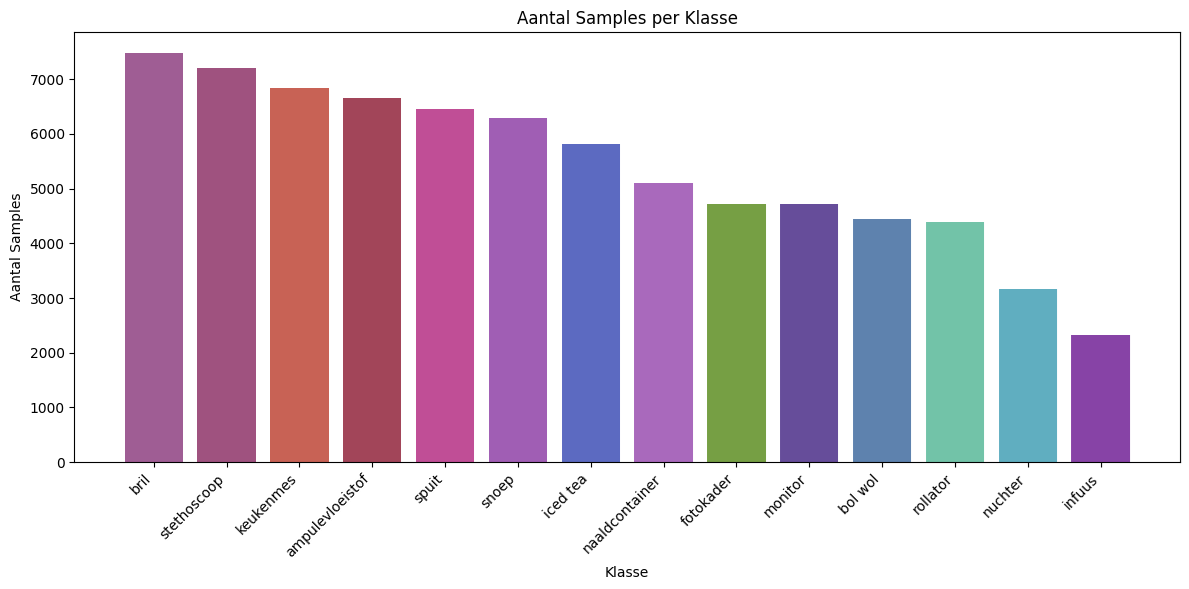
\includegraphics[width=1\textwidth]{samples-per-class.png}
    \caption[Aantal samples per klasse in de kalibratieopname]{
        \label{fig:samples-per-class}
        Aantal samples per klasse in de kalibratieopname.
        De getoonde aantallen zijn het resultaat van de tracking binnen de labeling tool.
      }
\end{figure}

Deze \texttt{per\_class\_metadata} dictionary wordt vervolgens doorgegeven aan de \texttt{create\_dataset} functie.

\paragraph{2. Selectie van Voorbeeldsamples per Klasse}
Om een gebalanceerde dataset te creëren voor training, en om de impact van de datasetgrootte te kunnen onderzoeken, 
werd per objectklasse een specifiek aantal voorbeeld-samples geselecteerd. 
De functie \texttt{select\_samples\_per\_class} implementeert deze selectie. 
Er werd geëxperimenteerd met verschillende aantallen samples per klasse: 500, 1000, 2000 en 3000 via de parameter \texttt{num\_samples\_per\_class}.
Indien een klasse onvoldoende unieke samples bevatte tegenover het opgegeven aantal, werd oversampling toegepast.
Alle beschikbare unieke samples werden eerste geselecteerd, waarna de resterende benodigde samples willekeurig met vervanging ui de beschikbare pool werden getrokken.

Met deze mapping, werden de train- en validatiesets gedefinieerd.
De functie \texttt{get\_train\_val\_split} verdeelt de geselecteerde samples in een train- en validatieset,
met een splitsing van 80\% voor training en 20\% voor validatie.
Deze stap resulteert in twee mappings: \texttt{train\_samples\_per\_class} en \texttt{val\_samples\_per\_class}.

Tenslotte werd ook per frame een lijst van \textit{alle} (dus niet enkel de geselecteerde) bounding boxes verzameld.
Dit is van belang omdat bij het maken van een crop rond een \textit{geselecteerd doelobject},
ook alle \textit{andere} objecten die toevallig in die crop vallen, correct gelabeld moeten worden voor de objectdetector.
De functie \texttt{get\_samples\_per\_frame} creëert hiertoe een dictionary (\texttt{all\_samples\_per\_frame}), 
waarbij elke frame-index gemapt wordt naar een lijst van alle objecten (klasse-ID en bounding box) die in dat frame voorkomen.

\paragraph{3. Genereren van Crops en YOLO-Labels voor Trainings- en Validatiesets}
Met de voorbereide lijsten van geselecteerde trainings- en validatiesamples per 
klasse (\texttt{train\_samples\_per\_class} en \texttt{val\_samples\_per\_class}) 
en de complete lijst van alle gelabelde objecten per frame (\texttt{all\_samples\_per\_frame}), 
kon de daadwerkelijke generatie van de dataset beginnen. 
Dit proces werd uitgevoerd door de functie \texttt{create\_train\_or\_val\_dataset}, 
die afzonderlijk werd aangeroepen voor het creëren van de trainingsdata en de validatiedata. 
De functie \texttt{create\_dataset} fungeerde als een overkoepelende wrapper die de mappenstructuur 
aanmaakte en de \texttt{create\_train\_or\_val\_dataset} functie aanriep (zie Codefragment{\ref{listing:create-train-val-dataset}}).

\begin{listing}[H]
  \fontsize{10pt}{9.6pt}
  \begin{minted}{python}
    def create_train_or_val_dataset(
      per_class_metadata,
      class_label_to_model_id,
      selected_samples_per_class,
      all_samples_per_frame,
      frames,
      images_path,
      labels_path,
      crop_size: int,
      is_validation=False,
  ):
      selected_samples_per_frame = get_selected_samples_per_frame(
          selected_samples_per_class
      )

      current_sample_idx = 0
      for frame_idx, frame in enumerate(tqdm(frames)):
          # check if the frame has any samples
          if selected_samples_per_frame.get(frame_idx) is None:
              continue

          image = cv2.imread(str(frame))

          # gather boxes and labels for the current frame
          class_ids, bboxes = zip(*all_samples_per_frame[frame_idx])
          bboxes = np.array(bboxes)
          class_labels = [
              per_class_metadata[class_id]["class_name"] for class_id in class_ids
          ]

          # for all selected samples in this frame, create crops
          for _, box in selected_samples_per_frame[frame_idx]:
              # create a crop for the current box
              transformed_image, transformed_bboxes, transformed_class_labels = create_crop_for_frame(
                  image,
                  crop_size,
                  box,
                  bboxes,
                  class_labels,
                  is_validation
              )

              # Save the transformed image and labels
              create_data_files(
                  labels_path,
                  images_path,
                  class_label_to_model_id,
                  current_sample_idx,
                  transformed_image,
                  transformed_bboxes,
                  transformed_class_labels,
              )

              current_sample_idx += 1
  \end{minted}
  \caption[Functie voor het creëren van de trainings- en validatiedatasets]{
    \label{listing:create-train-val-dataset}
    % TODO: Beschrijving
    }
\end{listing}




\subsubsection{Training van YOLOv11 Modellen}

\subsubsection{Combineren van Objectdetectie en FastSAM Tracking}

\section{Evaluatie van de Analysepipeline}

\section{Samenvatting van de Gehele Analysepipeline}